\documentclass{beamer}
\usepackage{movie15}
\usepackage{graphicx}
\usetheme{Copenhagen}

\title{Campus Mapper}
\author{Alex Hart\and Corey Young\and Dan Levy\and Jessica Perrie\and Mike McGuire}
\begin{document}

\begin{frame}
    \maketitle
\end{frame}

\begin{frame}{Introduction}
\begin{itemize}
    \item Created an app called CampusMapper for new Dalhousie students 
    \item Allow them to familiarize themselves with the campus
    \item Find different locations and activities in Halifax
    \item Developed in HTML and Javascript using jQueryMobile 
\end{itemize}
\end{frame}

\begin{frame}{Personas}
    \begin{columns}[c]
    \column{0.5 \textwidth}
        \center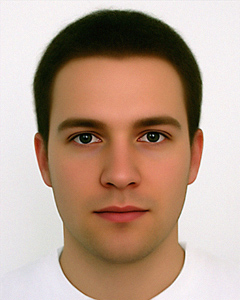
\includegraphics[height=0.5 \textheight]{bios/guy.jpg}
        \begin{itemize}
            \item Rob Smith
            \item 19 Years Old
            \item Canadian
            \item Not very tech savvy
        \end{itemize}
    \column{0.5 \textwidth}
        \center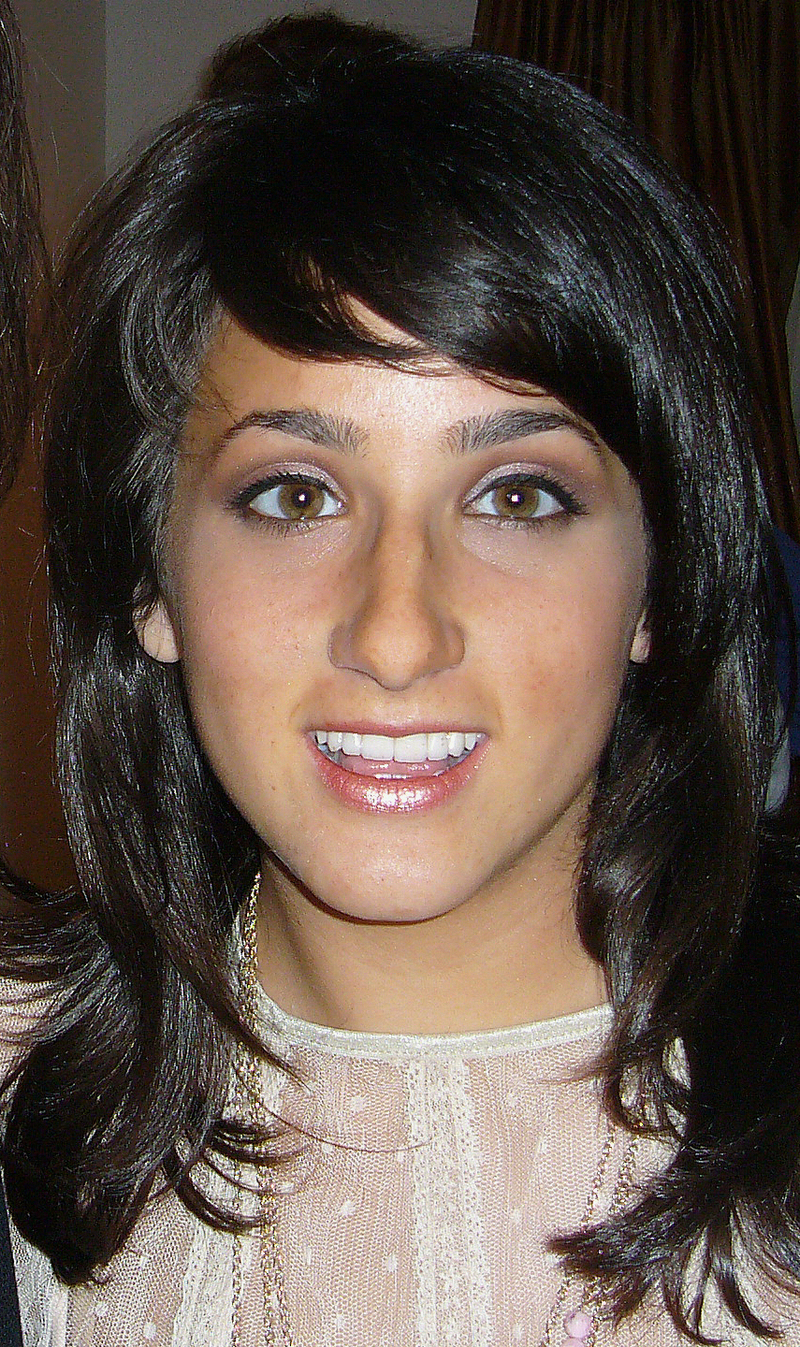
\includegraphics[height=0.5 \textheight]{bios/girl.jpg}
        \begin{itemize}
            \item Condoleezza Fernandez
            \item 23 Years Old
            \item Argentinian
            \item Familiar with technology
        \end{itemize}
    \end{columns}
\end{frame}

\begin{frame}{Tasks}
\begin{itemize}
    \item Use a social component to connect with friends
    \item Find a close wireless hot-spot
    \item Find a specific classroom on campus
    \item Receive notifications (tardiness, campus security, etc.)
    \item Bookmark a locations
    \item Find a local restaurant
\end{itemize}
\end{frame}

\begin{frame}{Tasks}
    \begin{block}{\center{Example Task}}
        \center{Find a Specific Classroom}
    \end{block}
\end{frame}

\begin{frame}{Find a Specific Classroom}
    \begin{columns}[c]
    \column{0.5 \textwidth}
        \center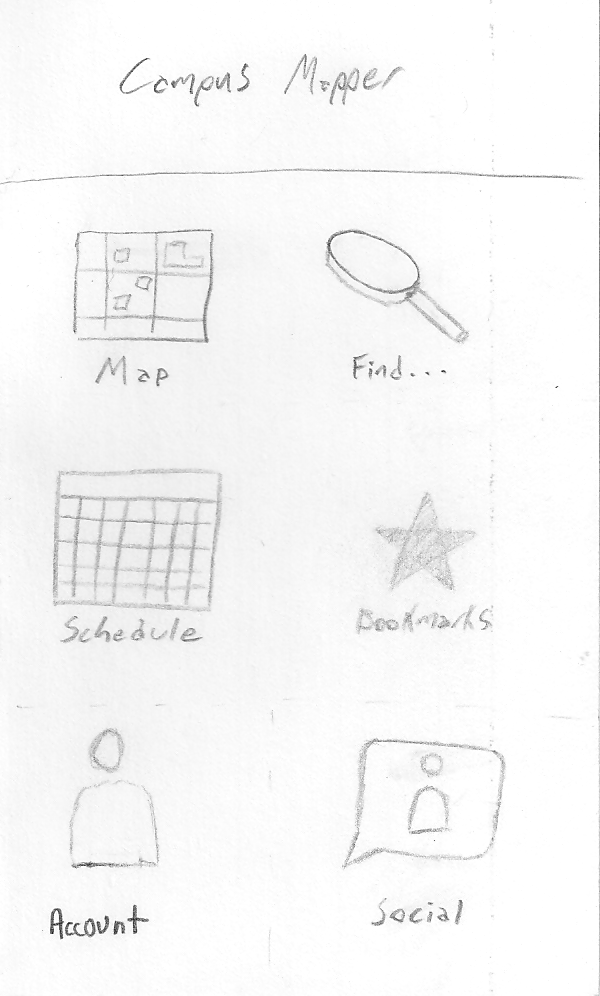
\includegraphics[height=0.75 \textheight]{hand-drawn/dashboard.png}
    \column{0.5 \textwidth}
        \begin{itemize}
            \item The application loads the Dashboard
            \item The user selects the Find icon
        \end{itemize}
    \end{columns}
\end{frame}

\begin{frame}{Find a Specific Classroom}
    \begin{columns}[c]
    \column{0.5 \textwidth}
        \center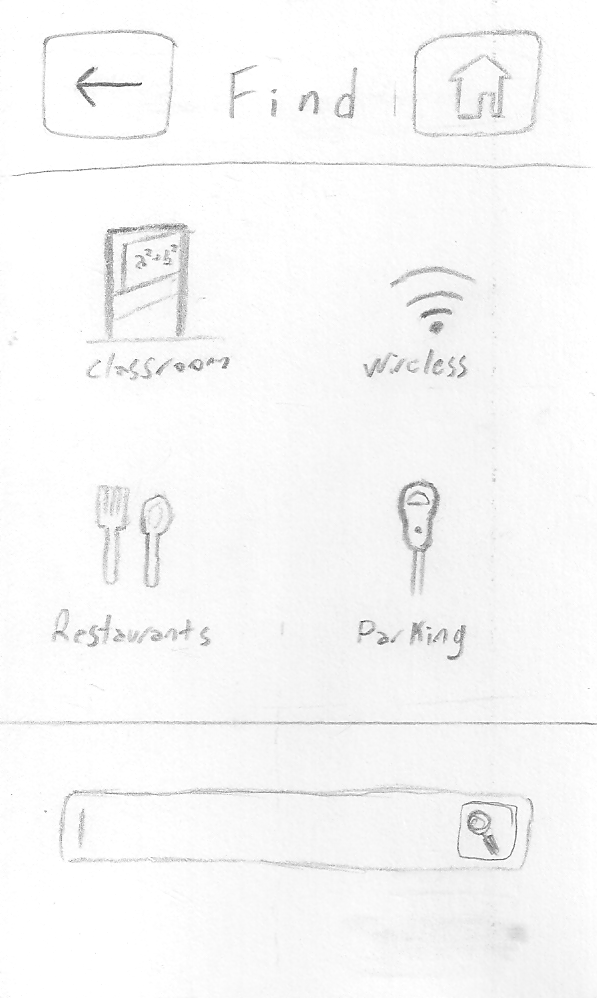
\includegraphics[height=0.75 \textheight]{hand-drawn/find.png}
    \column{0.5 \textwidth}
        \begin{itemize}
            \item The application shows the Find menu
            \item The user selects Classroom from the option grid
        \end{itemize}
    \end{columns}
\end{frame}

\begin{frame}{Find a Specific Classroom}
    \begin{columns}[c]
    \column{0.5 \textwidth}
        \center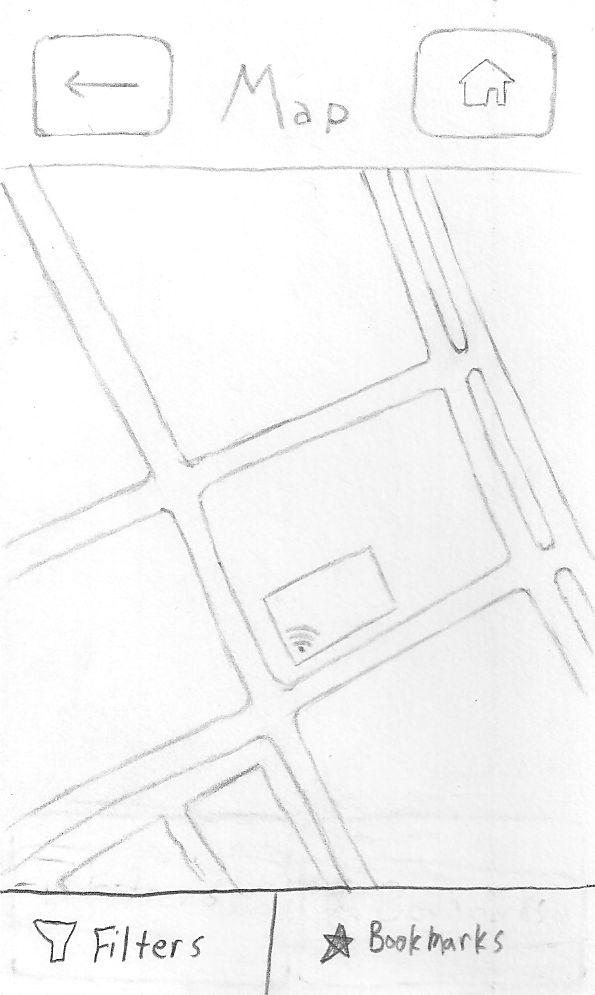
\includegraphics[height=0.75 \textheight]{hand-drawn/maps.png}
    \column{0.5 \textwidth}
        \begin{itemize}
            \item The application shows the Map screen highlighting the buildings on campus
            \item The user presses the desired building
        \end{itemize}
    \end{columns}
\end{frame}

\begin{frame}{Find a Specific Classroom}
    \begin{columns}[c]
    \column{0.5 \textwidth}
        \center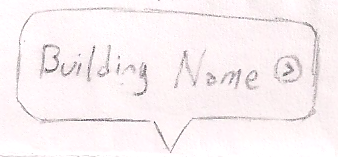
\includegraphics[width=\textwidth]{hand-drawn/map-popup.png}
    \column{0.5 \textwidth}
        \begin{itemize}
            \item The Map pop-up displays above the building showing the building name
            \item The user selects the pop-up
        \end{itemize}
    \end{columns}
\end{frame}

\begin{frame}{Find a Specific Classroom}
    \begin{columns}[c]
    \column{0.5 \textwidth}
        \center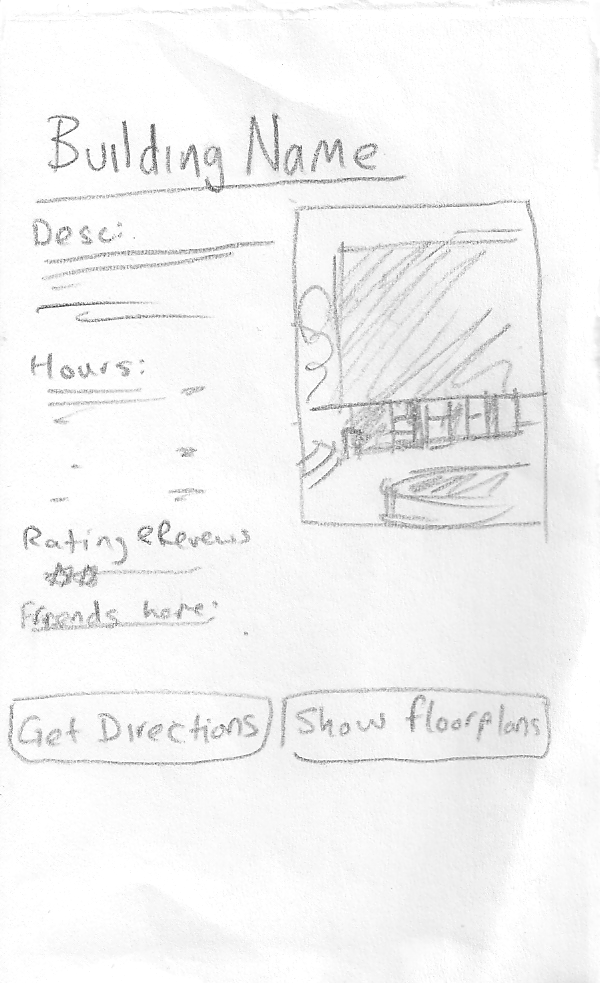
\includegraphics[height=0.75 \textheight]{hand-drawn/buildinginfo.png}
    \column{0.5 \textwidth}
        \begin{itemize}
            \item The system shows the Building Information screen
            \item The user selects Get Directions
        \end{itemize}
    \end{columns}
\end{frame}

\begin{frame}{Find a Specific Classroom}
    \begin{columns}[c]
    \column{0.5 \textwidth}
        \center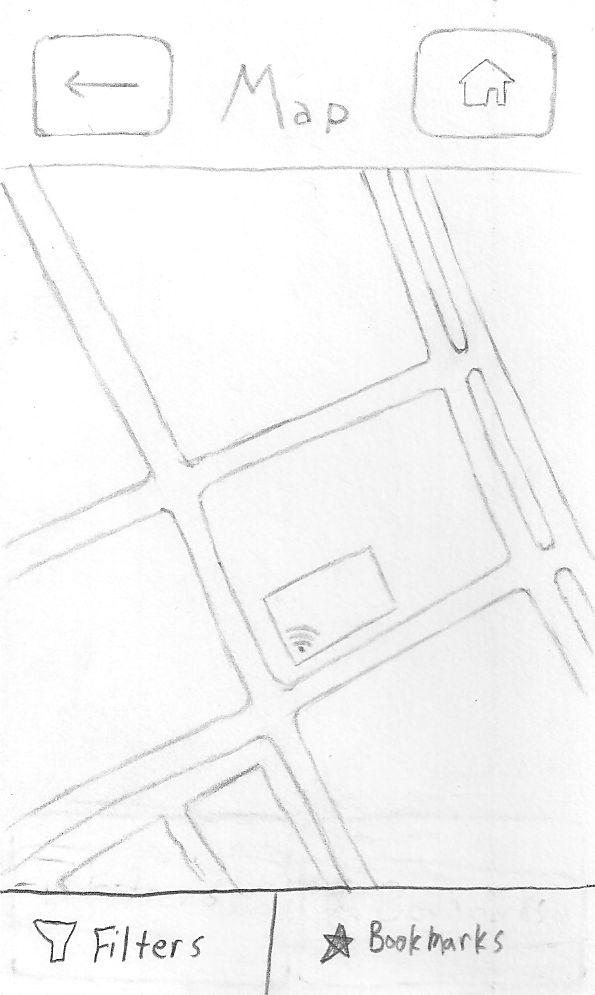
\includegraphics[height=0.75 \textheight]{hand-drawn/maps.png}
    \column{0.5 \textwidth}
        \begin{itemize}
            \item The system shows direction from the current location to the desired building
            \item The user can select the building pop-up at anytime to view a floor plan
        \end{itemize}
    \end{columns}
\end{frame}

\begin{frame}{Find a Specific Classroom}
    \begin{columns}[c]
    \column{0.5 \textwidth}
        \center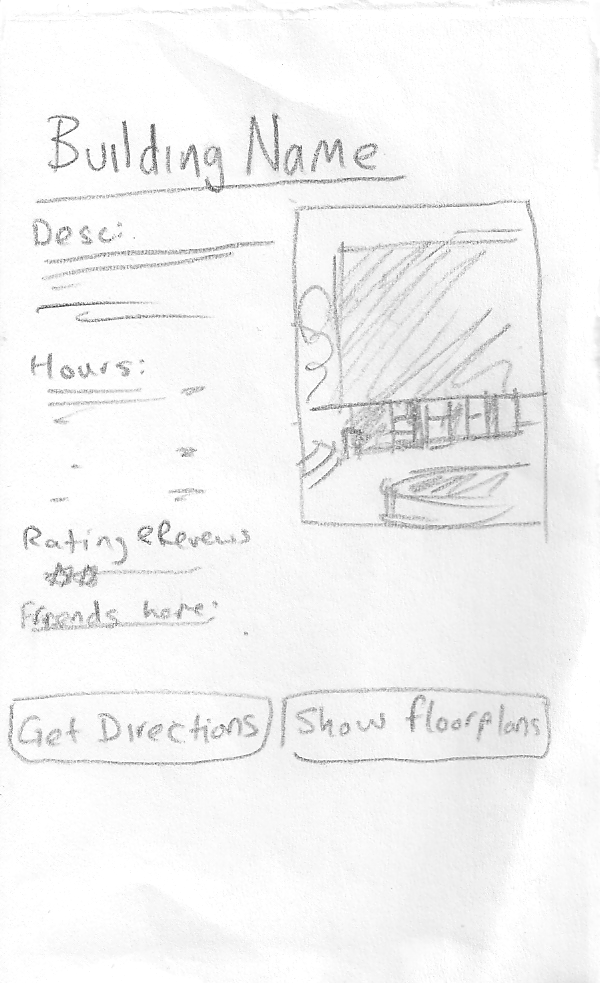
\includegraphics[height=0.75 \textheight]{hand-drawn/buildinginfo.png}
    \column{0.5 \textwidth}
        \begin{itemize}
            \item The system will display the Building Information screen
            \item The user can select Show Floor Plan
        \end{itemize}
    \end{columns}
\end{frame}

\begin{frame}{Find a Specific Classroom}
    \begin{columns}[c]
    \column{0.5 \textwidth}
        \center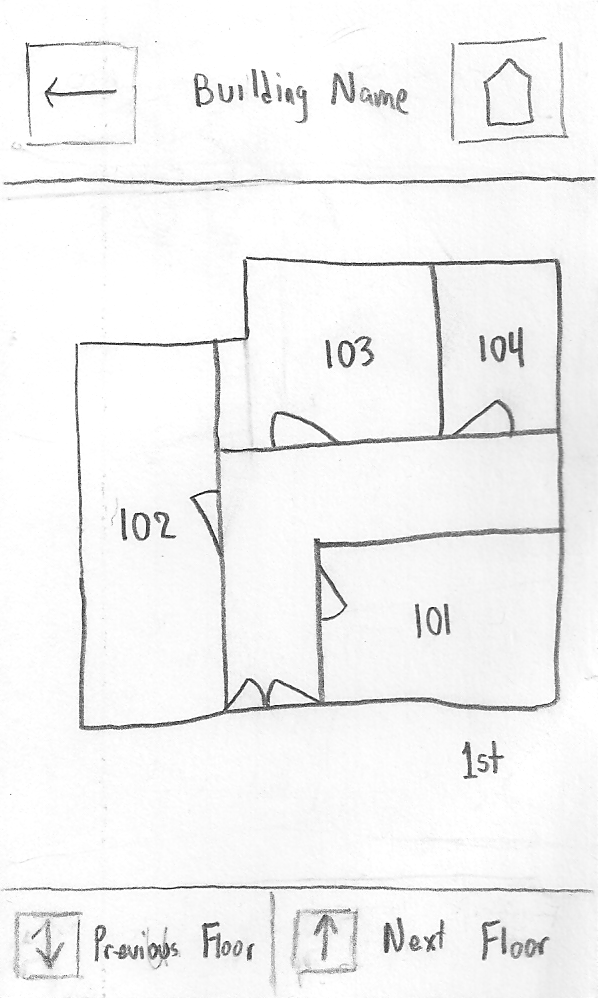
\includegraphics[height=0.75 \textheight]{hand-drawn/floorplan.png}
    \column{0.5 \textwidth}
        \begin{itemize}
            \item The user can see the floor plan and can move through different floors
        \end{itemize}
    \end{columns}
\end{frame}

\begin{frame}{Tasks}
    \begin{block}{\center{Social Task}}
        \center{See recent check-ins}
    \end{block}
\end{frame}

\begin{frame}{See Recent Check-ins}
    \begin{columns}[c]
    \column{0.5 \textwidth}
        \center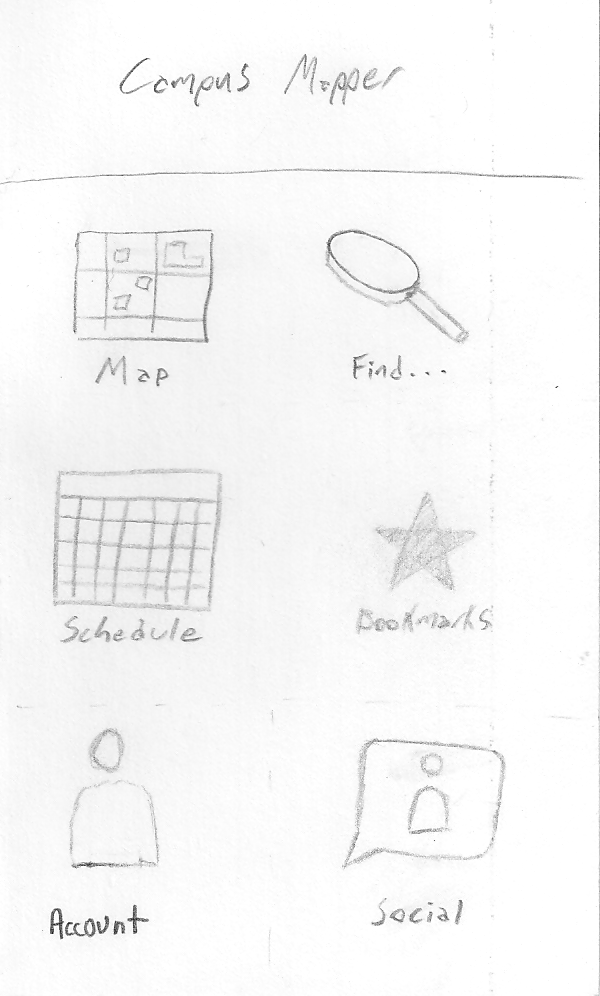
\includegraphics[height=0.75 \textheight]{hand-drawn/dashboard.png}
    \column{0.5 \textwidth}
        \begin{itemize}
            \item The application shows the Dashboard
            \item The user selects Social
        \end{itemize}
    \end{columns}
\end{frame}

\begin{frame}{See Recent Check-ins}
    \begin{columns}[c]
    \column{0.5 \textwidth}
        \center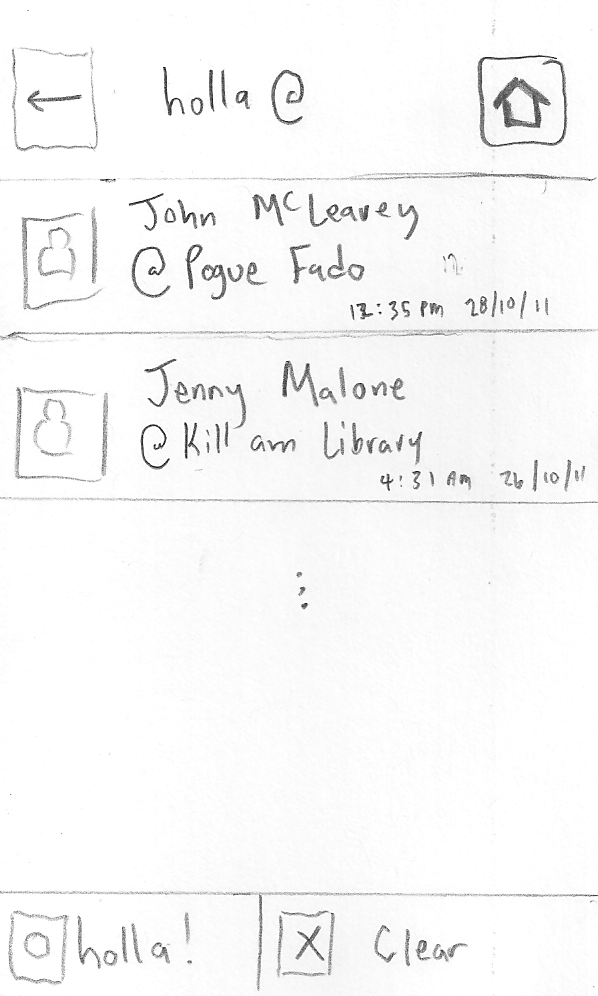
\includegraphics[height=0.75 \textheight]{hand-drawn/hollar.png}
    \column{0.5 \textwidth}
        \begin{itemize}
            \item The system displays a list of the users friends recent check-ins
        \end{itemize}
    \end{columns}
\end{frame}

\begin{frame}{Changes from Cognitive Walk Through}
    \begin{block}{Cognitive Walkthrough Results} 
    \begin{itemize}
        \item Several issues were brought to light
        \begin{itemize}
            \item Menu item ``Find'' not intuitive
            \item What was being bookmarked
            \item A Cluttered Map
        \end{itemize}
    \end{itemize}
    \end{block}
\end{frame}

\begin{frame}{Find not Intuitive}
    \begin{columns}[c]
    \column{0.5 \textwidth}
	    \center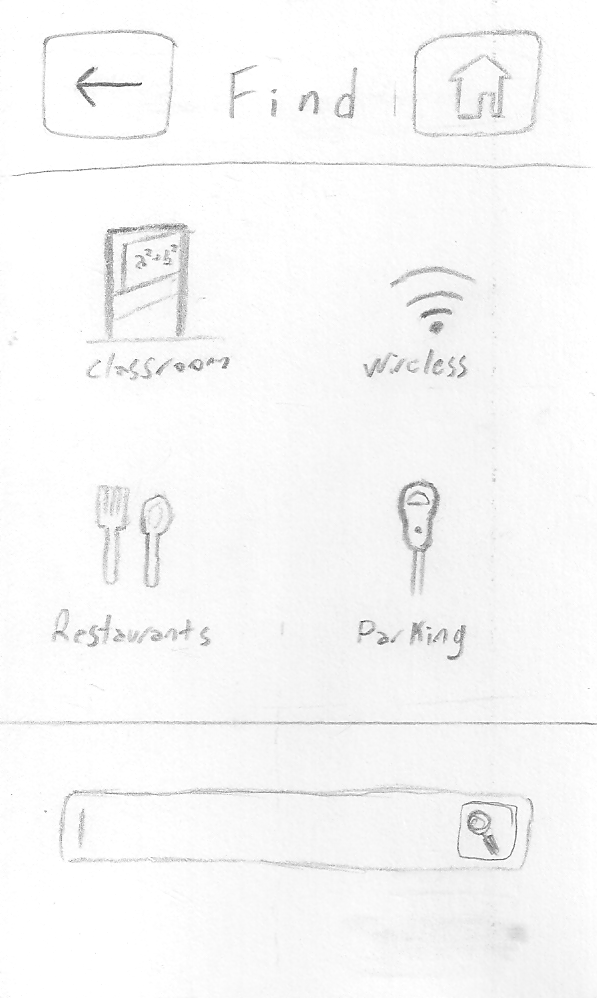
\includegraphics[height=0.5 \textheight]{hand-drawn/find.png}
    \column{0.5 \textwidth}
	    \center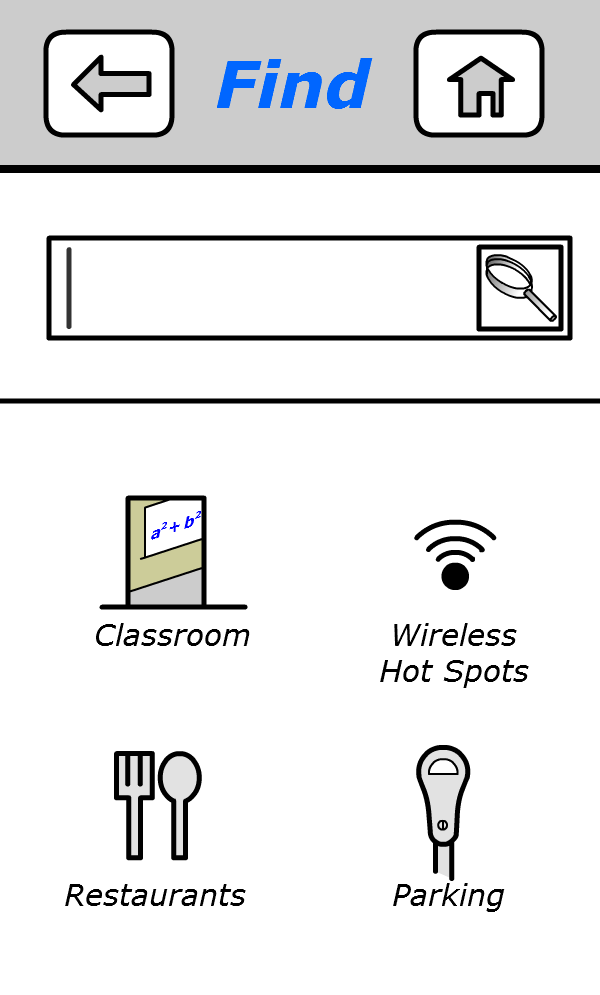
\includegraphics[height=0.5 \textheight]{digital/find.png}
    \end{columns}
    \begin{itemize}
        \item Removed Find from the dashboard
        \item Renamed it to Search Map and made it accessable from the Map screen
    \end{itemize}
\end{frame}

\begin{frame}{Bookmarks for What?}
    \begin{columns}[c]
    \column{0.5 \textwidth}
        \center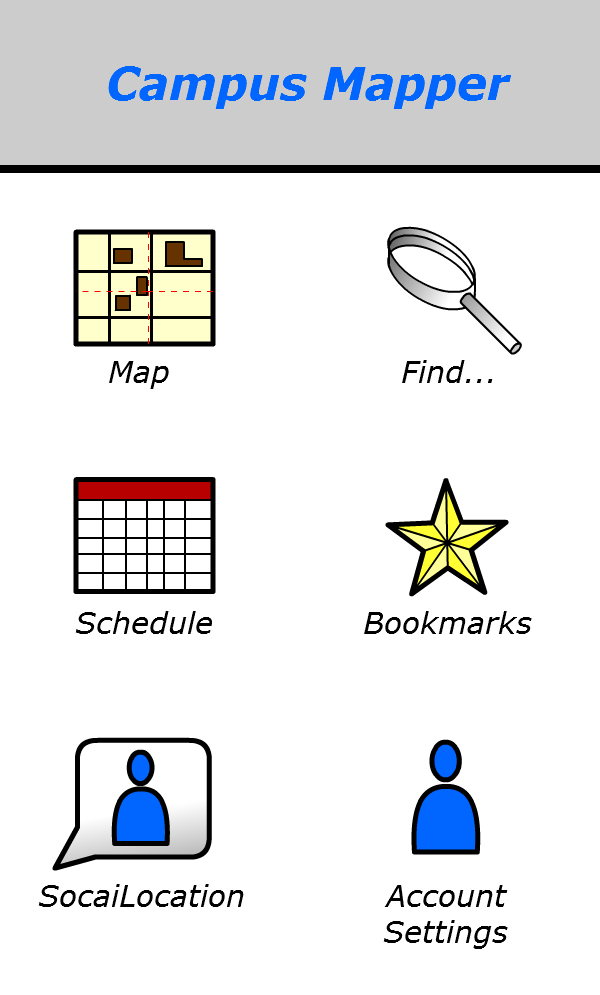
\includegraphics[height=0.5 \textheight]{digital/dashboard.png}
    \column{0.5 \textwidth}
        \center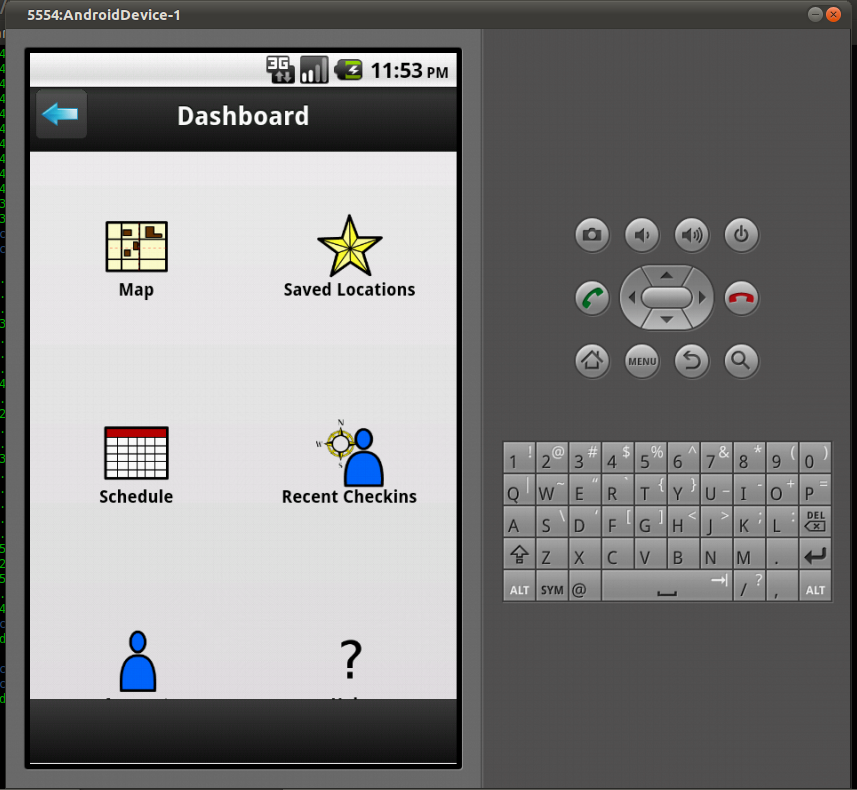
\includegraphics[height=0.5 \textheight]{final/dashboard.png}
    \end{columns}
    \begin{itemize}
        \item Renamed Bookmarks to Saved Locations
    \end{itemize}
\end{frame}

\begin{frame}{Markers are Confusing}
    \begin{columns}[c]
    \column{0.5 \textwidth}
        \center\includegraphics[height=0.5 \textheight]{digital/map_hotspots.png}
    \column{0.5 \textwidth} 
        \center\includegraphics[height=0.5 \textheight]{final/map_hotspots.png}
    \end{columns}
    \begin{itemize}
        \item changed from floating icons to icons in markers
    \end{itemize}
\end{frame}

\begin{frame}{Changes from the Heuristics Evaluation}
    \begin{block}{Heuristic Evaluation Results} 
    \begin{itemize}
        \item Several issues were brought to light
        \begin{itemize}
            \item Social How?
            \item TITLE 2
            \item TITLE 3
        \end{itemize}
    \end{itemize}
    \end{block}
\end{frame}

\begin{frame}{Social how?}
    \begin{columns}[c]
    \column {0.5 \textwidth}
        \center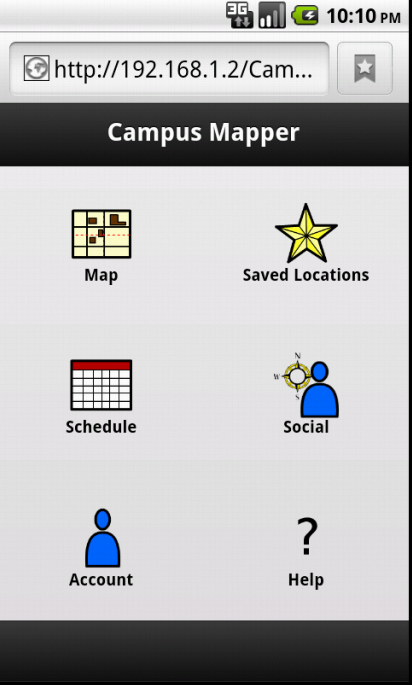
\includegraphics[height=0.5 \textheight]{final-pre-h/dashboard.png}
    \column {0.5 \textwidth}
        \center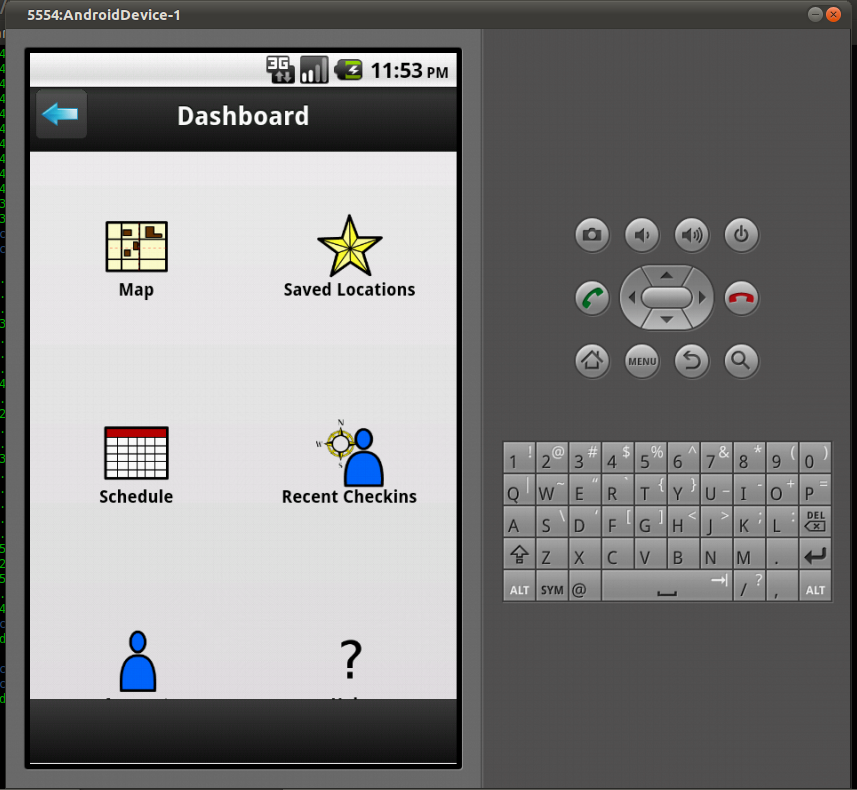
\includegraphics[height=0.5 \textheight]{final/dashboard.png}
    \end{columns}
    \begin{itemize}
        \item Changed Social to Check-ins for better recognition
    \end{itemize}
\end{frame}

\begin{frame}{TITLE 2}
    \begin{columns}[c]
    \column {0.5 \textwidth}
        \center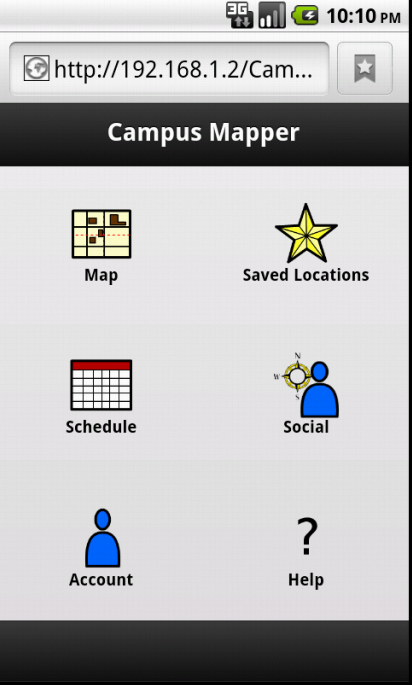
\includegraphics[height=0.5 \textheight]{final-pre-h/dashboard.png}
    \column {0.5 \textwidth}
        \center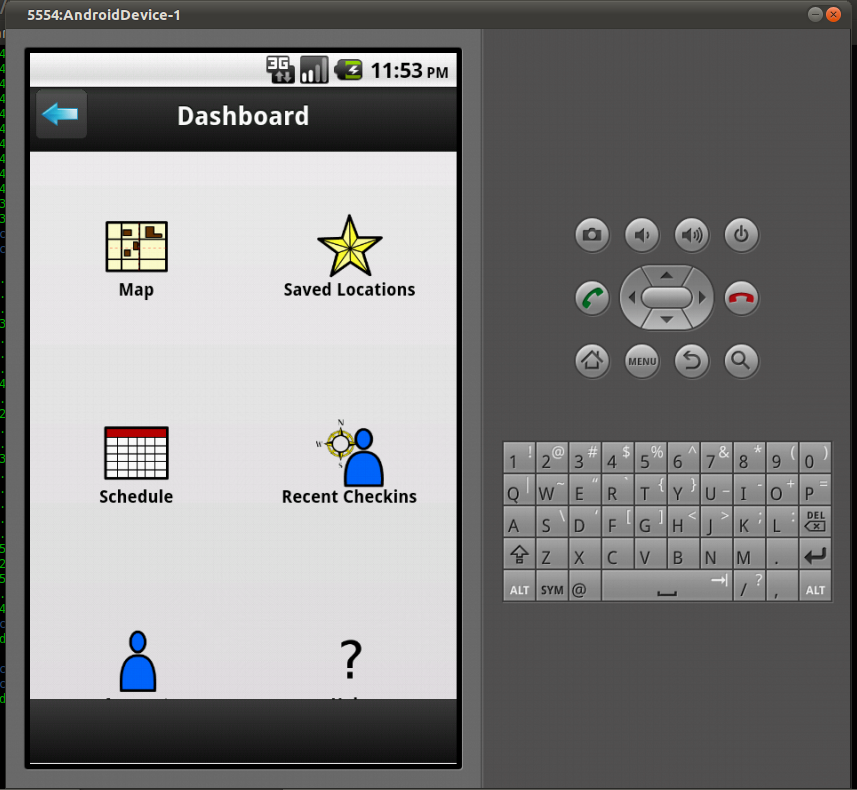
\includegraphics[height=0.5 \textheight]{final/dashboard.png}
    \end{columns}
    \begin{itemize}
        \item 
    \end{itemize}
\end{frame}

\begin{frame}{TITLE 3}
    \begin{columns}[c]
    \column {0.5 \textwidth}
        \center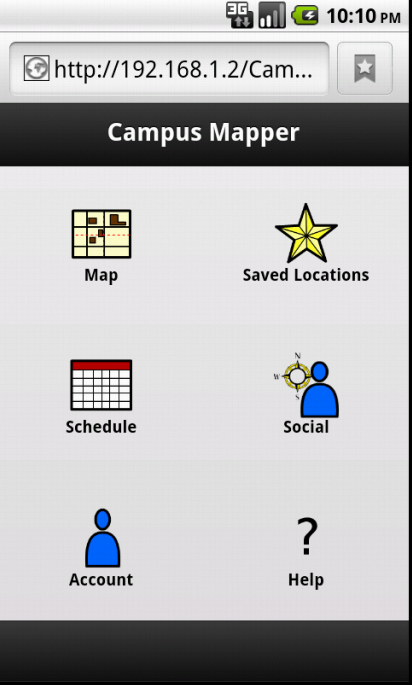
\includegraphics[height=0.5 \textheight]{final-pre-h/dashboard.png}
    \column {0.5 \textwidth}
        \center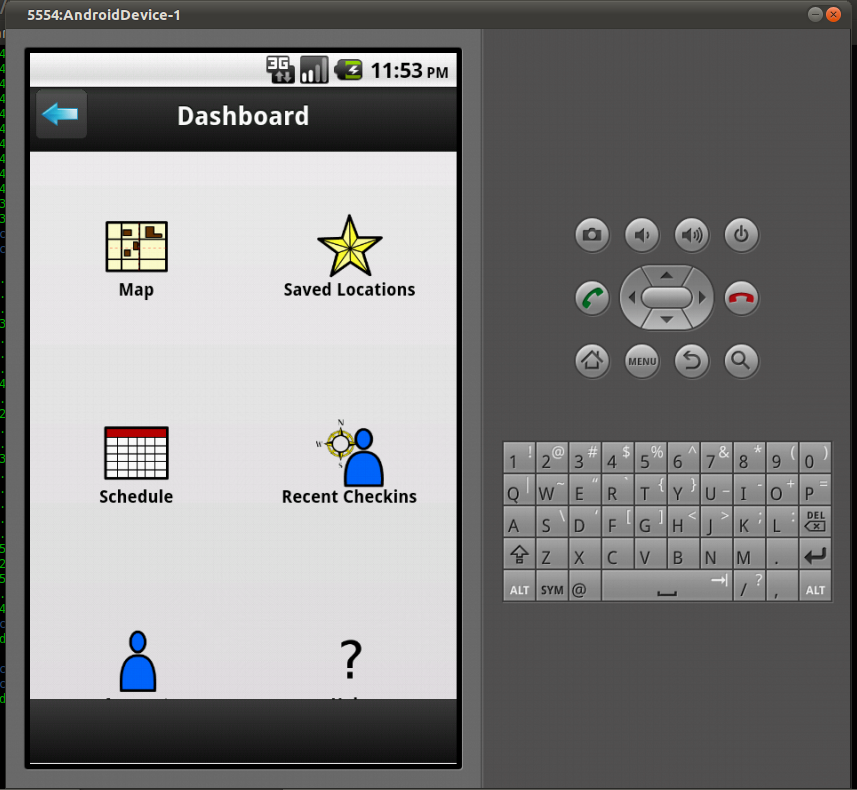
\includegraphics[height=0.5 \textheight]{final/dashboard.png}
    \end{columns}
    \begin{itemize}
        \item 
    \end{itemize}
\end{frame}

\begin{frame}{Video}
    \includemovie[poster,text={/small{Click to Play.}}]{\textwidth}{0.75 \textwidth}{video/UImovie.avi}
\end{frame}

\begin{frame}{Future Work \& Conclusions}
    \begin{itemize}
        \item General Debugging
        \item Add Breadcrumbs
        \item Add proper Help System
        \item Create new Layout - more appealing colors
        \item More User Interface Studies
    \end{itemize}
\end{frame}
\end{document}
